\documentclass[handout]{beamer}


\usetheme{default}
\usepackage{subfigure}
\usepackage{amsmath}
\usepackage{Sweave}
\usepackage{graphicx}
%\usepackage{color}
\usepackage{multicol}
\usepackage{bm}
\usepackage[all]{xy}
\usepackage{ulem}


\author{Patrick Lam}
\title{Bayesian Statistics in One Hour}
\date{}
%\date{April 23, 2009}

\setlength{\columnseprule}{.1pt}
\begin{document}

\newcommand{\red}{\textcolor{red}}
\newcommand{\blue}{\textcolor{blue}}
\newcommand{\purple}{\textcolor{purple}}
\newcommand{\brown}{\textcolor{brown}}
\newcommand{\cyan}{\textcolor{cyan}}

\frame{\titlepage}

\begin{frame}
\frametitle{Outline}
\tableofcontents
\end{frame}

\section{Introduction}

\begin{frame}
\frametitle{Outline}
\tableofcontents[currentsection]
\end{frame}

\begin{frame}
\frametitle{References}
\pause
\begin{figure}[!htp]
\begin{center}
\subfigure{\includegraphics[width=1in, height=1.5in]{gelman.jpg}}
\pause
\subfigure{\includegraphics[width=1in, height=1.5in]{gill.jpg}}
\pause
\subfigure{\includegraphics[width=1in, height=1.5in]{jackman.jpg}}
\end{center}
\end{figure}
\pause
\tiny
Western, Bruce and Simon Jackman.  1994.  ``Bayesian Inference for
Comparative Research.''  {\it American Political Science Review}
88(2): 412-423. \\
\bigskip
Jackman, Simon.  2000.  ``Estimation and Inference via Bayesian
Simulation: An Introduction to Markov Chain Monte Carlo.'' {\it
American Journal of Political Science} 44(2): 375-404. \\
\bigskip
Jackman, Simon.  2000. ``Estimation and Inference Are Missing Data
Problems: Unifying Social Science Statistics via Bayesian
Simulation.''  {\it Political Analysis} 8(4): 307-332. \\
\normalsize
\end{frame}

\begin{frame}[fragile]
\frametitle{Introduction}
\pause
Three general approaches to statistics:
\pause
\begin{itemize}
\item frequentist (Neyman-Pearson, hypothesis testing)
\pause
\item likelihood (what we've been learning all semester)
\pause
\item Bayesian
\end{itemize}
\pause
\bigskip
Today's goal: Contrast $\{$frequentist, likelihood$\}$ with Bayesian,
\pause with emphasis on Bayesian versus likelihood.\\
\pause
\bigskip
We'll go over some of the \emph{Bayesian critiques of
non-Bayesian analysis} \pause and {\it non-Bayesian critiques of Bayesian analysis}.
\end{frame}

\begin{frame}
\frametitle{Probability}
\pause
Objective view of probability (non-Bayesian):
\pause
\begin{itemize}
\item The relative frequency of an outcome of an experiment over
repeated runs of the experiment.
\pause
\item The observed proportion in a population.
\end{itemize}
\pause
\bigskip
Subjective view of probability (Bayesian):
\pause
\begin{itemize}
\item Individual's degree of belief in a statement
\pause
\item Defined personally \pause (how much money would you wager on an
outcome?)
\pause
\item Can be influenced in many ways (personal beliefs, prior evidence)
\end{itemize}
\pause
\bigskip
\emph{Bayesian statistics is convenient because it does not require
repeated sampling or large $n$ assumptions.} 
\end{frame}

\begin{frame}
\frametitle{Maximum Likelihood}
\pause
\begin{eqnarray*}
\blue{p(\theta | y)} &=& \frac{p(y | \theta) \red{p(\theta)} }{\brown{p(y)}} \\
&=& p(y| \theta) \purple{k(y)} \\
\pause
&\propto& p(y | \theta) \\\\
\pause
L(\theta | y) &=& p(y | \theta)\\
\end{eqnarray*}
\pause
There is a fixed, true value of $\theta$, \pause and we maximize the
likelihood to estimate $\theta$ and make assumptions to generate
uncertainty about our estimate of $\theta$.
\end{frame}

\begin{frame}
\frametitle{Bayesian}
\pause
\begin{eqnarray*}
\blue{p(\theta | y)} &=& \frac{p(y | \theta) \red{p(\theta)}
}{\brown{p(y)}} \\
\pause
&\propto& p(y | \theta) \red{p(\theta)}
\end{eqnarray*}
\pause
\begin{itemize}
\item $\theta$ is a random variable.
\pause
\begin{itemize}
\item $\theta$ is stochastic and changes from time to time.
\pause
\item $\theta$ is truly fixed, but we want to reflect our uncertainty
about it.
\end{itemize}
\pause
\item We have a \red{prior} subjective belief about $\theta$, which we
update with the data to form \blue{posterior} beliefs about $\theta$.
\pause
\item The \blue{posterior} is a probability
distribution that must integrate to 1.
\pause
\item The \red{prior} is usually a probability distribution that
integrates to 1 (proper prior). 
\end{itemize}
\end{frame}

\begin{frame}
\frametitle{$\theta$ as Fixed versus as a Random Variable}
\pause
Non-Bayesian approach ($\theta$ fixed):
\pause
\begin{itemize}
\item Estimate $\theta$ with measures of uncertainty (SE, CIs)
\pause
\item $95\%$ Confidence Interval: $95\%$ of the time, $\theta$ is in the
$95\%$ interval that is estimated each time.
\begin{itemize}
\pause
\item P($\theta \in 95\%$ CI$) = \pause$ 0 or 1  
\end{itemize}
\pause
\item P($\theta > 2) = \pause$ 0 or 1
\end{itemize}
\pause
\bigskip
Bayesian approach ($\theta$ random):
\pause
\begin{itemize}
\item Find the \blue{posterior} distribution of $\theta$.
\pause
\item Take quantities of interest from the distribution (posterior
mean, posterior SD, posterior credible intervals)
\pause
\item We can make probability statements regarding $\theta$.
\pause
\begin{itemize}
\item 95\% Credible Interval: \pause P($\theta \in$ 95\% CI) = 0.95
\pause
\item P($\theta > 2) = (0,1)$
\end{itemize} 
\end{itemize}
\end{frame}

\begin{frame}
\frametitle{Critiques}
\pause
\begin{eqnarray*}
\blue{\mathrm{Posterior}} &=& \mathrm{Evidence} \times \red{\mathrm{Prior}}
\end{eqnarray*}
\pause
NB: {\it Bayesians introduce \red{priors} that are not justifiable.} \\
\pause
\footnotesize B: \emph{Non-Bayesians are just doing Bayesian statistics with uninformative
priors, which may be equally unjustifiable.} \\
\bigskip
\pause
\normalsize
NB: {\it Unjustified Bayesian \red{priors} are driving the results.} \\
\pause
\footnotesize
B: \emph{Bayesian results $\approx$ non-Bayesian results as $n$ gets larger
(the data overwhelm the prior).} \\
\pause
\bigskip
\normalsize
NB: {\it Bayesian is too hard.  Why use it?} \\
\pause
\footnotesize
B: \emph{Bayesian methods allow us to easily estimate models that are too hard to
estimate (cannot computationally find the MLE) or unidentified (no unique MLE
exists) with non-Bayesian methods. \pause Bayesian methods also allow us to
incorporate prior/qualitative information into the model.}  
\normalsize
\end{frame}

\section{Bayesian Models}

\begin{frame}
\frametitle{Outline}
\tableofcontents[currentsection]
\end{frame}

\begin{frame}
\frametitle{Running a Model}
\pause
\begin{multicols}{2}
Non-Bayesian:
\pause
\begin{enumerate}
\item Specify a probability model (distribution for $Y$).
\pause
\item Find MLE $\hat{\theta}$ and measures of uncertainty (SE, CI).  Assume $\hat{\theta}$ follows a (multivariate) normal distribution.
\pause
\item Estimate quantities of interest analytically or via simulation.
\end{enumerate}
\newpage
\pause
Bayesian:
\begin{enumerate}
\item Specify a probability model (distribution for $Y$ and \red{priors} on
$\theta$).
\pause
\item Solve for \blue{posterior} and summarize it (mean, SD, credible
interval, etc.).  We can do both analytically or via simulation.
\pause
\item Estimate quantities of interest analytically or via simulation.
\end{enumerate}
\end{multicols}
\emph{There is a Bayesian way to do any non-Bayesian
parametric model.}
\end{frame}

\begin{frame}
\frametitle{A Simple (Beta-Binomial) Model}
\pause
The Los Angeles Lakers play 82 games during a regular NBA season.
\pause In the 2008-2009 season, they won 65 games.  \pause Suppose the Lakers win each
game with probability $\pi$.  \pause Estimate $\pi$. \\
\pause
\bigskip
We have 82 Bernoulli observations or one observation $Y$, where
\begin{eqnarray*}
Y \sim \mathrm{Binomial}(n, \pi)
\end{eqnarray*}
with $n=82$.\\
\bigskip
\pause
Assumptions:
\pause
\begin{itemize}
\item Each game is a Bernoulli trial.
\pause
\item The Lakers have the same probability of winning each game.  
\pause
\item The outcomes of the games are independent.
\end{itemize}
\end{frame}

\begin{frame}
We can use the beta distribution as a \textcolor{red}{prior} for
$\pi$ since it has support over [0,1].
\pause
\footnotesize
\begin{eqnarray*}
\textcolor{blue}{p(\pi | y)} &\propto& p(y | \pi) \textcolor{red}{p(\pi)} \\
\pause
&=& \mathrm{Binomial}(n, \pi) \times
\textcolor{red}{\mathrm{Beta}(\alpha, \beta)}\\
\pause
&=& \binom{n}{y} \pi^y (1 - \pi)^{(n-y)} \textcolor{red}{\frac{\Gamma (\alpha + \beta)}{\Gamma (\alpha)
\Gamma (\beta)} \pi^{(\alpha - 1)} (1 - \pi)^{(\beta-1)}}\\
\pause
&\propto& \pi^y (1 - \pi)^{(n-y)} \textcolor{red}{\pi^{(\alpha - 1)}
(1 - \pi)^{(\beta-1)}} \\\\
\pause
\textcolor{blue}{p(\pi | y)} &\textcolor{blue}{\propto}& \textcolor{blue}{\pi^{y+\alpha-1} (1-\pi)^{n-y+\beta-1}}
\end{eqnarray*}
\normalsize
\pause
The \textcolor{blue}{posterior} distribution is simply a
\textcolor{blue}{Beta($y+\alpha, n-y+\beta$)} distribution. \pause
Effectively, our \textcolor{red}{prior} is just adding $\alpha-1$
successes and $\beta - 1$ failures to the dataset.\\
\bigskip
\pause
{\it Bayesian \red{priors} are just adding pseudo observations to the data.}
\end{frame}

\begin{frame}
Since we know the \blue{posterior} is a \blue{Beta($y+\alpha, n-y+\beta$)}
distribution, we can summarize it analytically or via simulation with
the following quantities:
\pause
\bigskip
\begin{itemize}
\item posterior mean
\pause
\item posterior standard deviation
\pause 
\item posterior credible intervals (credible sets)
\pause
\item highest posterior density region
\end{itemize} 
\end{frame}

\begin{frame}




\begin{figure}[!htp]
\subfigure{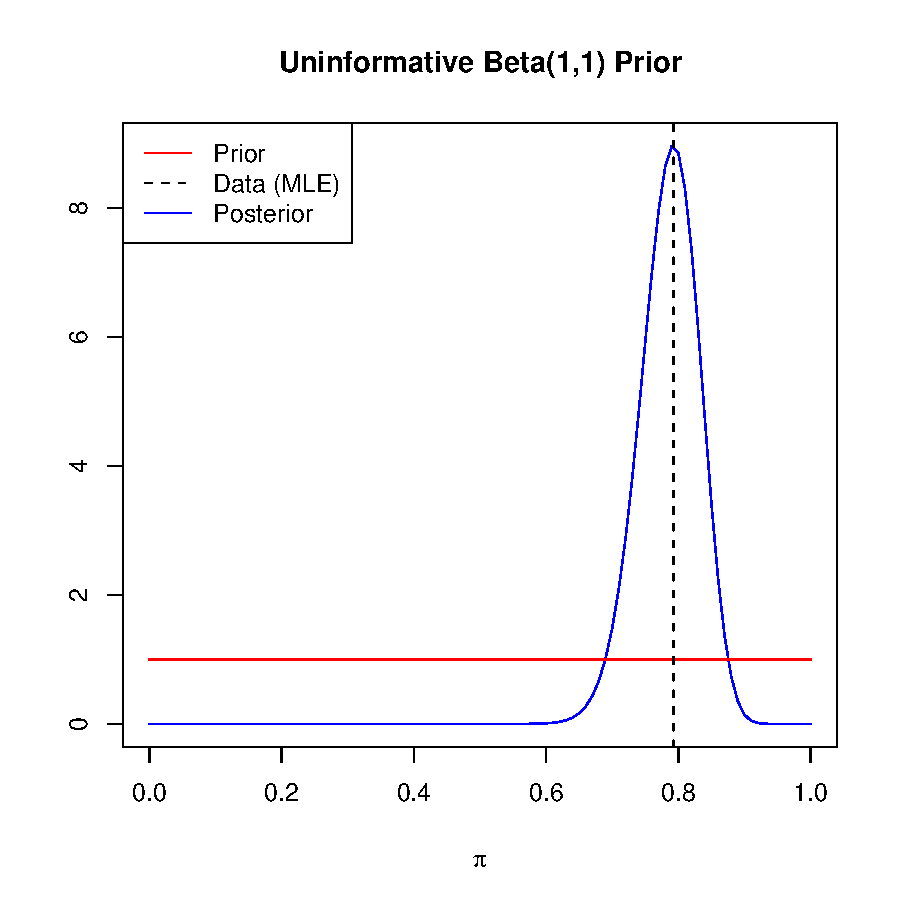
\includegraphics[width=1.5in, height=1.5in]{bayesianhour-prior1.pdf}}
\subfigure{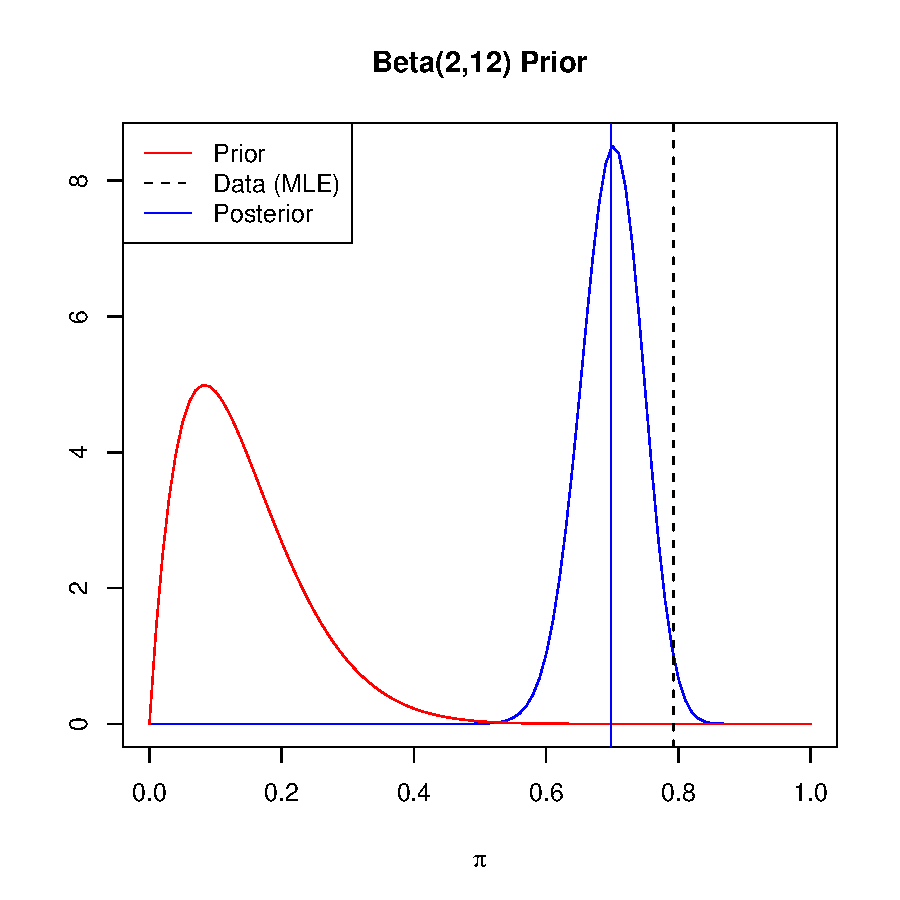
\includegraphics[width=1.5in, height=1.5in]{bayesianhour-prior2.pdf}}\\
\subfigure{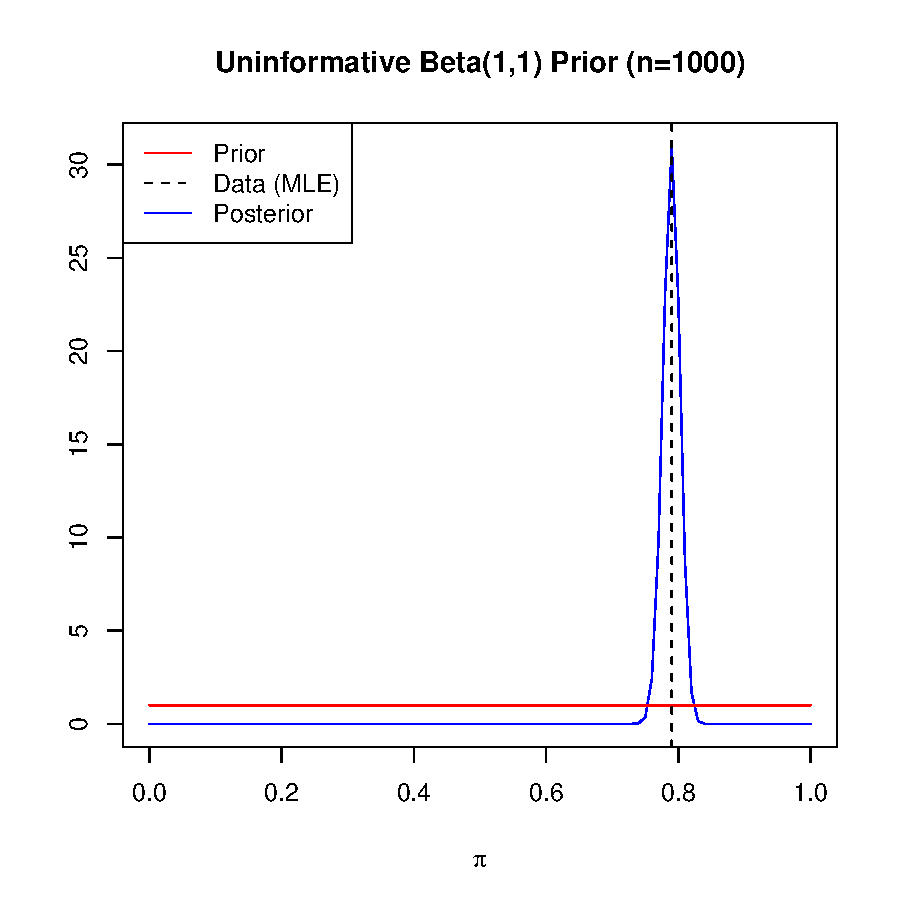
\includegraphics[width=1.5in, height=1.5in]{bayesianhour-prior3.pdf}}
\subfigure{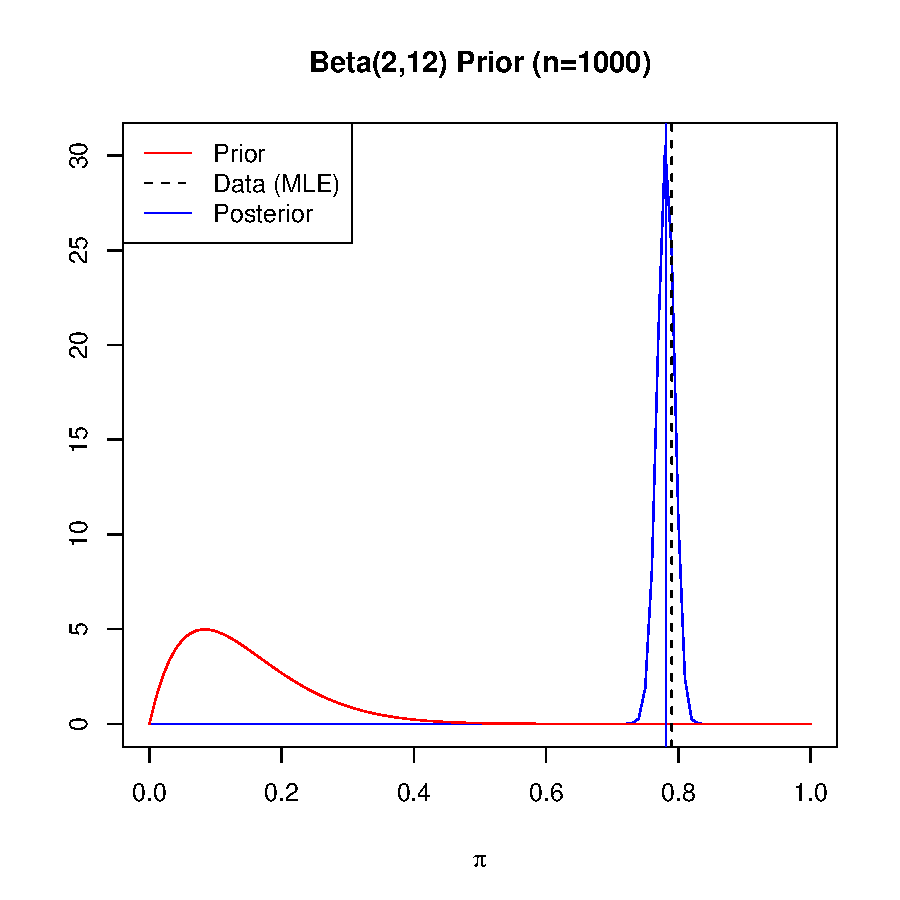
\includegraphics[width=1.5in, height=1.5in]{bayesianhour-prior4.pdf}}
\end{figure}
\end{frame}

\begin{frame}
In the previous model, we had
\footnotesize
\begin{eqnarray*}
\blue{\mathrm{Beta}(y+\alpha, n-y+\beta)} &=& \frac{\mathrm{Binomial}(n, \pi) \times
\red{\mathrm{Beta}(\alpha, \beta)}}{\brown{p(y)}}\\
\end{eqnarray*}
\normalsize
\pause
We knew that the likelihood $\times$ \red{prior} produced something
that looked like a Beta distribution up to a \brown{constant} of
proportionality. \\
\pause
\bigskip
Since the \blue{posterior} must be a probability distribution, we know
that it is a Beta distribution and we can easily solve for the
\brown{normalizing constant} \pause (although we don't need to since we
already have the \blue{posterior}). \\
\bigskip
\pause
When the \blue{posterior} is the same distribution family as the
\red{prior}, we have {\bf conjugacy}. \\
\bigskip
\pause
Conjugate models are great because we can find the exact
\blue{posterior}, \pause but we almost never have conjugacy except in
very simple models.
\end{frame}

\begin{frame}
\frametitle{What Happens When We Don't Have Conjugacy?}
\pause
Consider a Poisson regression model with Normal priors on
$\bm{\beta}$.
\pause
\footnotesize
\begin{eqnarray*}
\blue{p(\bm{\beta} | \mathbf{y})} &\propto& \prod_{i=1}^n
\mathrm{Poisson}(\lambda_i) \times \red{\mathrm{Normal}(\bm{\mu},
\bm{\Sigma})}\\
\pause
\lambda_i &=& \exp(\bm{x_i \beta})\\\\
\pause
\blue{p(\bm{\beta} | \mathbf{y})} &\propto& \prod_{i=1}^n
\frac{\exp(-e^{\bm{x_i \beta}}) \exp(\bm{x_i \beta})^{y_i}}{y_i!}
\times \\
&\phantom{\propto}& \red{\frac{1}{(2\pi)^{d/2} |\bm{\Sigma}|^{1/2}}
\exp\left(\frac{1}{2} (\bm{\beta} - \bm{\mu})^T \bm{\Sigma}^{-1} (\bm{\beta} - \bm{\mu})\right)}\\
\end{eqnarray*}
\normalsize
\pause
Likelihood $\times$ \red{prior} doesn't look like any distribution we
know (non-conjugacy) \pause and \brown{normalizing constant} is too hard to find, \pause
so how do we find our \blue{posterior}?
\end{frame}

\begin{frame}
\frametitle{MCMC to the Rescue}
\pause
Ideal Goal: \pause Produce {\bf independent} draws from our \blue{posterior}
distribution via simulation and summarize the \blue{posterior} by using those
draws. \\
\pause
\bigskip
\purple{Markov Chain} \cyan{Monte Carlo} (\purple{MC}\cyan{MC}): a
class of algorithms that produce \purple{a chain} of \cyan{simulated draws} from a distribution
where \purple{each draw is {\bf dependent} on the previous draw}. \\
\pause
\bigskip
Theory: \pause If our chain satisfies some basic conditions, then the chain
will {\bf eventually converge} to a stationary distribution (in our case, the
\blue{posterior}) \pause and we have approximate draws from the
\blue{posterior}.\\
\pause
\bigskip
{\it But there is no way to know for sure whether our chain has converged.}
\end{frame}

\begin{frame}
\frametitle{Algorithm 1: Gibbs Sampler}
\pause
Let $\bm{\theta}^t = (\theta_1^t, \dots, \theta_k^t)$ be the $t$th
draw of our parameter vector $\bm{\theta}$.\\
\pause
\bigskip
Draw a new vector $\bm{\theta}^{t+1}$ from the following distributions:
\pause
\begin{eqnarray*}
\theta_1^{t+1} &\sim& p(\theta_1 | \theta_2^t, \dots, \theta_k^t,
\bm{y}) \\
\pause
\theta_2^{t+1} &\sim& p(\theta_2 | \theta_1^{t+1}, \dots, \theta_k^t,
\bm{y}) \\
\pause
&\vdots&\\
\pause
\theta_k^{t+1} &\sim& p(\theta_k | \theta_1^{t+1}, \dots, \theta_{k-1}^{t+1},\bm{y}) \\
\end{eqnarray*}
\pause
Repeat $m$ times to get $m$ draws of our parameters from the
approximate \blue{posterior} (assuming convergence). \\
\pause
\bigskip
Requires that we know the conditional distributions for each
$\theta$.  \pause What if we don't?
\end{frame}

\begin{frame}
\frametitle{Algorithm 2: Metropolis-Hastings}
\pause 
Draw a new vector $\bm{\theta}^{t+1}$ in the following way:
\pause
\begin{enumerate}
\item Specify a jumping distribution $J_{t+1}(\bm{\theta}^* |
\bm{\theta}^{t})$ \pause (usually a symmetric distribution such as the multivariate normal).
\pause
\item Draw a proposed parameter vector $\bm{\theta}^*$ from the jumping
distribution. 
\pause
\item Accept $\bm{\theta}^*$ as $\bm{\theta}^{t+1}$ with probability
min(r,1), where 
\pause
\begin{eqnarray*}
r = \frac{p(\bm{y}|\bm{\theta}^*) \red{p(\bm{\theta}^*)}}{p(\bm{y}|\bm{\theta}^{t}) \red{p(\bm{\theta}^{t})}}
\end{eqnarray*}
\pause
If $\bm{\theta}^*$ is rejected, then $\bm{\theta}^{t+1} = \bm{\theta}^t$.
\end{enumerate}
\pause
\bigskip
Repeat $m$ times to get $m$ draws of our parameters from the
approximate \blue{posterior} (assuming convergence). \\
\pause
\bigskip
M-H always works, but can be very slow.\\
\end{frame}

\section{Applications}

\begin{frame}
\frametitle{Outline}
\tableofcontents[currentsection]
\end{frame}

\subsection{Missing Data}

\begin{frame}
\frametitle{Missing Data}
\pause
Suppose we have missing data.  \pause Define $D$ as our data matrix
and $M$ as our missingness matrix.
\pause
\setlength{\columnseprule}{0pt}
\begin{multicols}{2}
$$
D = \left( \begin{array}{cccc}
y & x_1 & x_2 & x_3\\
1 & 2.5 & 432 & 0 \\
5 & 3.2 & 543 & 1 \\
2 & ? & 219 & ? \\
? & 1.9 & ? & 1  \\
? & 1.2 & 108 & 0 \\
? & 7.7 & 95 & 1 \\
\end{array} \right)
$$
\newpage
$$
M = \left( \begin{array}{cccc}
y & x_1 & x_2 & x_3\\
1 & 1 & 1 & 1 \\
1 & 1 & 1 & 1 \\
1 & 0 & 1 & 0 \\
0 & 1 & 0 & 1  \\
0 & 1 & 1 & 1 \\
0 & 1 & 1 & 1 \\
\end{array} \right)
$$
\end{multicols}
\pause
\bigskip
One non-Bayesian approach to dealing with missing data is {\bf
multiple imputation}.
\end{frame}

\begin{frame}
\frametitle{Multiple Imputation}
\pause
We need a method for filling in the missing cells of $D$ as a first
step {\bf before} we go to the analysis stage. 
\bigskip
\pause
\begin{enumerate}
\item Assume a joint distribution for $D_{obs}$ and $M$:
\pause
\begin{eqnarray*}
p(D_{obs}, M | \phi, \gamma) = \int p(D | \phi) p(M |
D_{obs}, D_{mis}, \gamma) dD_{mis} \\
\end{eqnarray*}
\pause
If we assume MAR, then 
\begin{eqnarray*}
p(D_{obs}, M | \phi, \gamma) &\propto& \int p(D | \phi) dD_{mis} \\
\end{eqnarray*}
\end{enumerate}
\end{frame}

\begin{frame}
\begin{enumerate}
\item[2.] Find $\phi$, which characterizes the full $D$.
\pause
\begin{eqnarray*}
L(\phi | D_{obs}) &=& \prod_{i=1}^n \int p(D_{i,obs} | \phi) dD_{mis} \\
\end{eqnarray*}
\pause
How do we do this integral? \\
\pause
\bigskip
Assume Normality since the marginals of a multivariate Normal are Normal.
\pause
\begin{eqnarray*}
L(\mu, \Sigma | D_{obs}) &=& \prod_{i=1}^n N(D_{i,obs} | \mu_{obs},
\Sigma_{obs}) 
\end{eqnarray*}
\pause
\item[3.] Find $\hat{\mu}, \hat{\Sigma}$ and its distribution via EM algorithm and bootstrapping.
\pause
\item[4.] Draw $m$ $\mu, \Sigma$ values, then use them to predict values for $D_{mis}$.
\end{enumerate}
\end{frame}

\begin{frame}
What we end up with is $m$ datasets with missing values imputed. \\
\pause
\bigskip
We then run our regular analyses on the $m$ datasets and combine the
results using Rubin's rule.
\end{frame}

\begin{frame}
\frametitle{Bayesian Approach to Missing Data}
\pause
Bayesian paradigm: Everything unobserved is a random variable.\\
\bigskip
\pause
So we can set up the missing data as a ``parameter'' that we need to find.
\pause
\begin{eqnarray*}
\blue{p(D_{mis}, \phi, \gamma | D_{obs}, M)} &\propto& p(D_{obs}| D_{mis}
, \phi) p(D_{mis}|\phi) p(M | D_{obs}, D_{mis}, \gamma) \\
&\phantom{\propto} &\red{p(\gamma) p(\phi)}
\end{eqnarray*}
\pause
If we assume MAR:
\pause
\begin{eqnarray*}
\blue{p(D_{mis}, \phi, \gamma | D_{obs}, M)} \propto p(D_{obs}| D_{mis}
, \phi) p(D_{mis}|\phi) \red{p(\phi)}\\
\end{eqnarray*}
\pause
Use Gibbs Sampling or M-H to sample both $D_{mis}$ and $\phi$.\\
\pause
\bigskip
We don't have to assume normality of $D$ to integrate over
$D_{mis}$. \pause We can just drop the draws of $D_{mis}$.
\end{frame}

\begin{frame}
We can also incorporate both imputation and analyses in the same model.
\begin{eqnarray*}
\blue{p(\bm{\theta}, D_{mis}, \phi, \gamma | D_{obs}, M)} &\propto&
p(\bm{y}_{obs}, \bm{y}_{mis} | \bm{\theta}) p(D_{obs}| D_{mis}
, \phi)p(D_{mis}|\phi) \\
&\phantom{\propto}&  \red{p(\phi) p(\bm{\theta})}\\
\end{eqnarray*}
\pause
Again, find the \blue{posterior} via Gibbs Sampling or M-H. \\
\bigskip
\pause
Moral: We can easily set up an application specific Bayesian model to
incorporate missing data.
\end{frame}

\subsection{Hierarchical Models}

\begin{frame}
\frametitle{Multilevel Data}
\pause
Suppose we have data in which we have $i = 1, \dots, n$ observations
that belong to one of $j = 1, \dots, J$ groups. \\
\pause
\bigskip
Examples:
\pause 
\begin{itemize}
\item students within schools
\pause
\item multiple observations per country
\pause
\item districts within states
\end{itemize}
\pause
\bigskip
We can have covariates on multiple levels.  \pause How do we deal with this
type of data?
\end{frame}

\begin{frame}
\frametitle{The Fixed Effects Model}
\pause
We can let the intercept $\alpha$ vary by group:
\pause
\begin{eqnarray*}
y_i = \alpha_{j[i]} + x_{i1} \beta_1 + x_{i2} \beta_2 + \epsilon_i\\
\end{eqnarray*}
\pause
\bigskip
This is known as the {\bf fixed effects} model.  \\
\pause
\bigskip
This is equivalent to estimating dummy variables for $J-1$ groups. \\
\pause
\bigskip
We can use this model if we think that there is something inherent about the
groups that affects our dependent variable. \\
\pause
\bigskip
However, the fixed effects model involves estimating many parameters,
and also cannot take into account group-level covariates.
\end{frame}

\begin{frame}
\frametitle{Hierarchical Model}
\pause
A more flexible alternative is to use a {\bf hierarchical model}, also
known as a multilevel model, mixed effects model, or random effects model.
\pause
\begin{eqnarray*}
y_i &=& \alpha_{j[i]} +  x_{i1} \beta_1 + x_{i2} \beta_2 + \epsilon_i\\
\pause
\alpha_{j} &\sim& N(\alpha, \sigma^2_{\alpha}) \\
\end{eqnarray*}
\pause
Instead of assuming a completely different intercept for each group,
we can assume that the intercepts are drawn from a common (Normal) distribution.
\end{frame}

\begin{frame}
We can incorporate group-level covariates in the following way:
\pause
\begin{eqnarray*}
y_i &=& \alpha_{j[i]} +  x_{i1} \beta_1 + x_{i2} \beta_2 + \epsilon_i\\
\pause
\alpha_{j} &\sim& N(\gamma_0 + u_{j1} \gamma_1, \sigma^2_{\alpha}) \\
\end{eqnarray*}
\pause
or equivalently
\pause 
\begin{eqnarray*}
y_i &=& \alpha_{j[i]} +  x_{i1} \beta_1 + x_{i2} \beta_2 + \epsilon_i\\
\pause
\alpha_{j} &=& \gamma_0 + u_{j1} \gamma_1 + \eta_j \\
\pause
\eta_j &\sim& N(0, \sigma^2_{\alpha}) \\
\end{eqnarray*}
\pause
This is a relatively difficult model to estimate using non-Bayesian
methods.  The {\tt lme4()} package in R can do it.
\end{frame}

\begin{frame}
\frametitle{Bayesian Hierarchical Model}
\pause
\begin{eqnarray*}
y_i &=& \alpha_{j[i]} +  x_{i1} \beta_1 + x_{i2} \beta_2 + \epsilon_i\\
\pause
\alpha_{j} &\sim& N(\gamma_0 + u_{j1} \gamma_1, \sigma^2_{\alpha}) \\
\end{eqnarray*}
\pause
We can do hierarchical models easily using Bayesian methods.
\pause
\begin{eqnarray*}
\blue{p(\bm{\alpha}, \bm{\beta}, \bm{\gamma}|\bm{y})} &\propto& p(\bm{y}
| \bm{\alpha}, \bm{\beta}, \bm{\gamma})
\red{p(\bm{\alpha}|\bm{\gamma}) p(\bm{\gamma}) p(\bm{\beta})} \\
\end{eqnarray*}
\pause
Solve for the joint \blue{posterior} using Gibbs Sampling or M-H. \\
\pause
\bigskip
We incorporate data with more than two levels easily as well.
\end{frame}

\begin{frame}
\frametitle{Conclusion}
\pause
There are pros and cons to using Bayesian statistics.
\pause
\bigskip
\begin{multicols}{2}
Pros:
\pause
\begin{itemize}
\item Incorporate outside/prior knowledge
\pause
\item Estimate much more difficult models
\pause
\item CI have more intuitive meaning
\pause
\item Helps with unidentified models
\end{itemize}
\newpage
\pause
Cons:
\pause
\begin{itemize}
\item It's hard(er)
\pause
\item Computationally intensive
\pause
\item Need defense of priors
\pause
\item No guarantee of MCMC convergence
\end{itemize}
\end{multicols}
Statistical packages for Bayesian are also less developed ({\tt
MCMCpack()} in R, WinBUGS, JAGS).
\end{frame}

\subsection{Item-Response Models}

\end{document}

